Dalam pembuatan aplikasi Oracle Apex Online, anda juga dapat memodifikasi source HTML dan CSS yang anda inginkan untuk mempercantik antarmuka penggunaan aplikasi.
\section{Pengertian HTML}
Hypertext Markup Language adalah sebuah bahasa pemrograman yang diciptakan untuk membuat program tampilan halaman web dasar, pada HTML juga terdiri dari beberapa kode yang biasa diawali dengan kurung siku buka dan diakhiri dengan kurung siku tutup.
\par dalam program HTML sangatlah sederhana tidak serumit dengan PHP atau bahasa lainnya, HTML berguna untuk menciptakan Interface atau Antarmuka pengguna dengan aplikasi web, biasanya bidang FRONT-end Developer saja yang ditugaskan untuk merancang aplikasi namun.
\par HTML juga ada beberapa jenis, misalnya HTML5 yaitu web antarmuka yang Responsive dengan segala macam device baik dari komputer,laptop,sampai pada mobile device, HTML5 biasanya ditambahkan dengan Bootstrap JS(Javascript) maupun Bootstrap CSS(Cascading Style Sheet) yaitu perantara agar dapat memberikan antarmuka yang sempurna dalam membuat web HTML5
\par Adapun kode sederhana yang dipakai dalam penggunaan bahasa HTML sebagai berikut:
\begin{lstlisting}
<!DOCTYPE html>
<html>
<head>
<title>Titel Halaman</title>
</head>
<body>

<h1>Ini adalah heading</h1>
<p>Ini adalah Paragraf.</p>

</body>
</html>
\end{lstlisting}

\section{Pengertian CSS}
Cascading Style Sheet adalah sebuah perantara bahasa pemrograman yang digunakan untuk menambahkan atribut pada kode HTML, dalam pembuatan HTML biasanya menggunakan CSS yang berguna untuk mempercantik atau mempermudah interaksi dengan pengguna website.
\par Dalam CSS juga anda dapat mengatur atribut dan juga fungsi-fungsi yang digunakan pada kode HTML misalkan memperbaiki tampilan, mengubah warna, memperbaiki tata letak sebuah kode seperti div page, dan banyak lagi.
\par Kode sederhana CSS yang digunakan pada HTML adalah sebagai berikut:
\begin{lstlisting}
<!DOCTYPE html>
<html>
<head>
<style>
body {background-color: green;}
h1   {color: blue;}
p    {color: red;}
</style>
</head>
<body>

<h1>Ini adalah heading</h1>
<p>Ini adalah paragraf.</p>

</body>
</html>
\end{lstlisting}

\par Untuk menyatukannya kita menggunakan script HTML dan CSS, kita akan membuat sebuah STATIC CONTENT tentang halaman About Us, yang dimana menampil-kan profil kami pada sebuah halaman website, kodenya seperti berikut:

\begin{lstlisting}
<style type="text/css">
#kiri
{
width:50%;
height:100%;
float:left;
}
#kanan
{
width:50%;
height:100%;
float:right;
}
img{
border-radius:70%;
}
</style>

<div id="kiri"><center>
  <h3>Rizaluardi Achmad Pratama</h3>
  <p>1184102
  <p><img width="25%" height="25%" src="...isi dengan source gambar....">

</center></div>

<div id="kanan"><center>
    <h3>M Ichsam Kurniawan Nasution</h3>
    <p>1184110
    <p><img width="25%" height="25%" src="....isi dengan source gambar...">
</center></div>
\end{lstlisting}

\par berikut adalah contoh dari kode CSS yang tergabung dalam HTML, buatlah kode tersebut untuk mengetahui step selanjutnya.

\section{Menggabungkan HTML dengan CSS dan Memasukan pada Aplikasi}
Untuk memasukkannya kita ikuti langkah langkah berikut :
\begin{enumerate}
    
    \begin{figure}
	\item Buatlah STATIC CONTENT pada halaman TEST PAGE yang sudah dibuat sebelumnya, anda bisa menemukannya pada Regions lalu pilih Static Content, lihat pada Gambar 11.1.
	
        \centering
        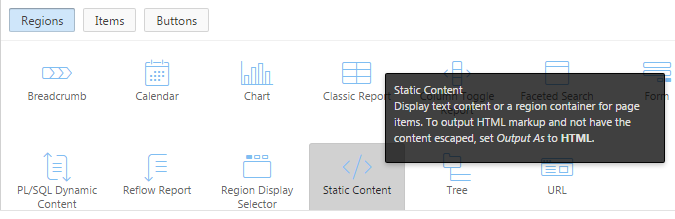
\includegraphics[scale=0.5]{figures/bab11/1.png}
        \caption{\textit{Static Content}}
        \label{Static Content}
    \end{figure}
    
    \begin{figure}
    \item Tarik Static Content menuju Content Body , lihat pada Gambar 11.2.
        
        \centering
        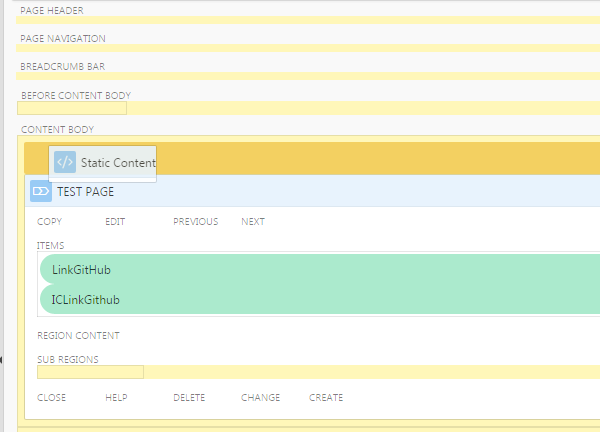
\includegraphics[scale=0.5]{figures/bab11/2.png}
        \caption{\textit{Static Content 2}}
        \label{Static Content 2}
    \end{figure}
    
    \begin{figure}
    \item Lalu buatlah title dengan nama About Us, setelah itu pada menu source akan terlihar text, disitulah yang nantinya akan dimasukkan kode dari HTML dan CSS klik tombol yang ditandai warna merah, lihat pada Gambar 11.3.
    
        \centering
        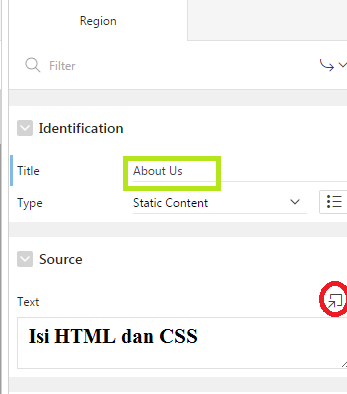
\includegraphics[scale=0.5]{figures/bab11/3.png}
        \caption{\textit{Static Content 3}}
        \label{Static Content 3}
    \end{figure}
    
    \begin{figure}
    \item Lalu masukkan kode yang telah dibuat tadi ke Code Editor berikut pastikan isikan source gambar yang anda inginkan, lihat pada Gambar 11.4.
        
        \centering
        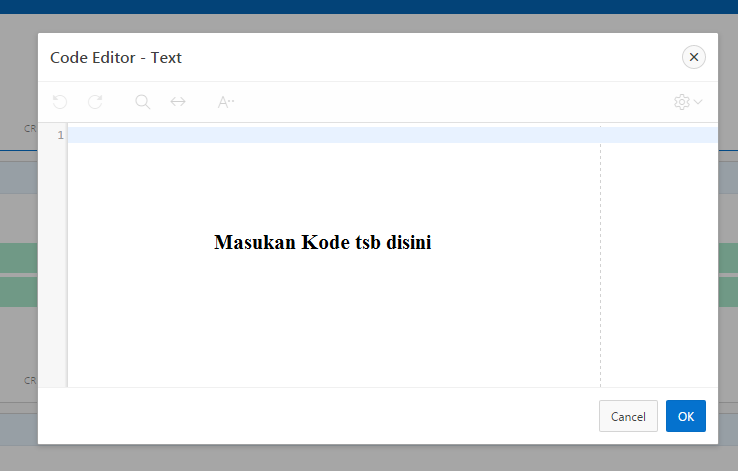
\includegraphics[scale=0.5]{figures/bab11/4.png}
        \caption{\textit{Static Content 4}}
        \label{Static Content4}
    \end{figure}
    
    \begin{figure}
    \item Berikut adalah Tampilan jika kita memasukkan HTML dan CSS pada aplikasi Oracle Apex menggunakan Static Content, lihat pada Gambar 11.5.
        
        \centering
        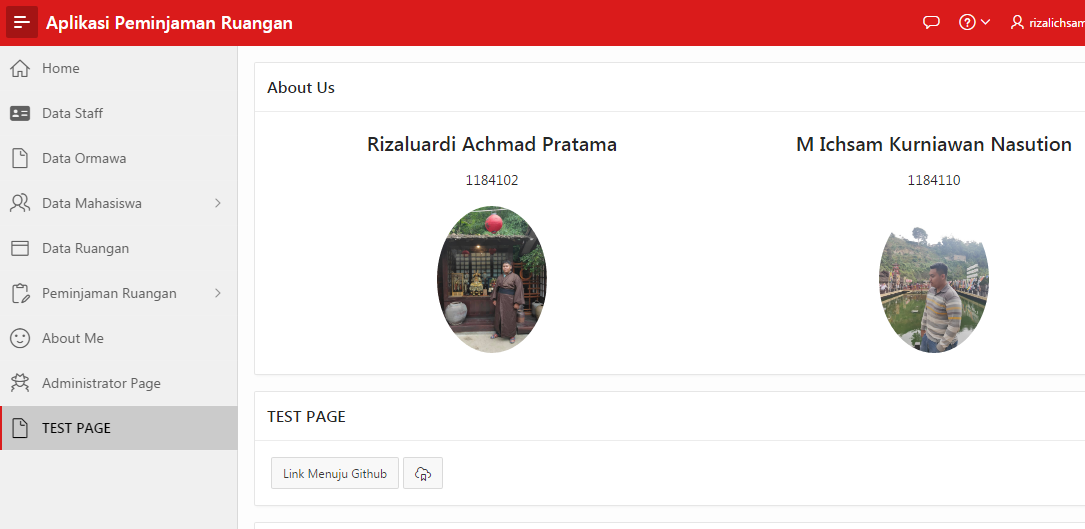
\includegraphics[scale=0.4]{figures/bab11/5.png}
        \caption{\textit{Hasil Static Content}}
        \label{Static Content5}
    \end{figure}
    
    
\end{enumerate}